\documentclass[../../main.tex]{subfiles}

\begin{document}

\section{Introduction}

Steganography is the technique of hiding a message inside another message or a
physical object.\cite{steganography-definition}
The word \emph{steganography} comes from the Greek word
\emph{steganographia}, which is the combination of \emph{steganós} meaning
``covered'' and \emph{-graphia} meaning ``writing''.

The first testimonials of the use of steganography date back to 440 BC in Greece
mentioned by Herodotus in his \emph{Histories}: Histitateus sent a message to
Aristagoras by writing a text message on the shaved head of one of his servants
and then waited till the hair of the servant had regrow to sent him to
Aristagoras.
Moreover steganography has been used for centuries in different ways such as
secret inks, morse code hidden inside physical objects or encoded in eyes
blinking (Jeremiah Denton, tortured prisoner-of-war in 1966 during the korean
war, encoded in this way an help message during a TV report) or microdots
embedded in paper or in clothes used by espionage agents during and after the
World War II.

In digital steganography a message or a file is concealed within another file;
in particular, electronic communications may contain a steganographic coding
inside a information vehicle such as a document, a program or a media file
(image, audio or video).
Media files are ideal for hiding messages since due to their large size, the
modification needed to encode a steganographic coding cause a subtle change that
is unlikely to notice for someone who is not looking for it.
This is one of the greatest differences of steganography with respect to
cryptography: in cryptography the encrypted messages are visible so they attract
interest and it's more likely that they will be subject to some type of attacks
to be decoded.

In this paper we will focus on steganalysis, the study of detecting and, if
possible, recovering hidden messages encoded using steganography, the way in
which it can be performed, examples of its application in known cases and
the threats and opportunities regarding the cybersecurity implications of its
use in digital and communications systems.

We can call steganalysis successful (and consequentially that the steganography
is broken) when there is the evidence of an hidden message in the cover signal.
Moreover, the embedded information can also be crypted, in that case the
attacker (the one who tries to find the hidden message) will have to perform
cryptanalysis in order to decrypt the information.

The Field on Information Security Systems is indeed vast and will require much
more space than the one we have. Here we attach a map which describes shortly
the structure.

\begin{figure}[h]
    \centering
    \caption{Map of Information Security Systems \cite{modern-text-hiding}}
    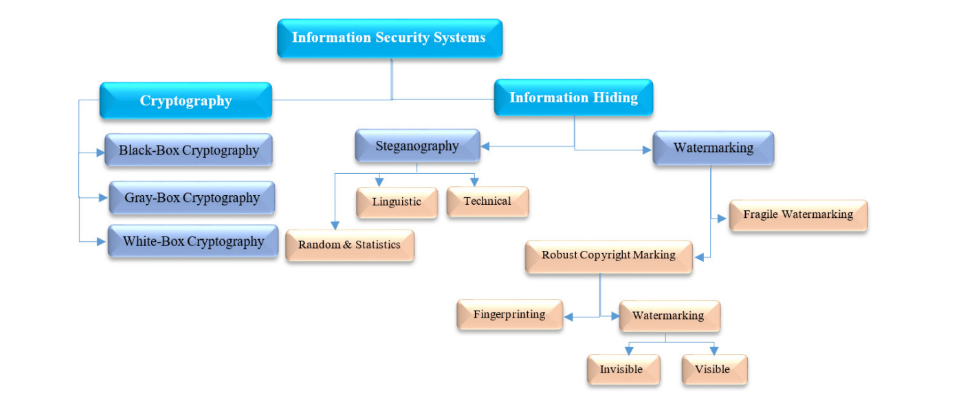
\includegraphics[scale=0.65]{map.png}
\end{figure}

\pagebreak

\end{document}